\documentclass[a4paper]{exam}

\usepackage{amsfonts,amsmath,amsthm}
\usepackage{geometry}
\usepackage{tikz}


\title{Problem Set 15: Graphs and Matchings}
\author{CS/MATH 113 Discrete Mathematics}
\date{Spring 2024}

\usepackage{draftwatermark}
\SetWatermarkText{Sample Solution}
\SetWatermarkScale{3}
\SetWatermarkLightness{.95}

\boxedpoints

\printanswers

\begin{document}
\maketitle

The problems below make use of concepts and definitions from Sections 10.1 and 10.2 in our textbook. Solving the problems will be tremendously easier if you have gone over the sections and the worked examples included therein, browsed the end-of-section exercises, and consulted their solutions at the back of the book. If you are still stuck at some problem, feel free to consult course staff during their consultation hours as shared on Canvas.

\begin{questions}
  
  \question Prove that a connected graph with $n$ vertices has at least 2 vertices of the same degree.
    \begin{solution}
      This is a false statement and cannot be proved. We provide a counterexample below.

    \begin{proof} The claim is false.

      Here is a connected graph with $n=2$ vertices. No 2 vertices have the same degree.
      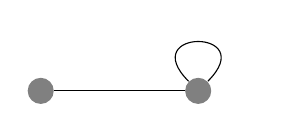
\begin{tikzpicture}
        \node[fill,circle, gray] at (0,0) (a) {};
        \node[fill,circle, gray] at (2,0) (b) {};

        \draw[-] (a) -- (b);
        \draw (b) to [out=135,in=45,looseness=10] (b);
      \end{tikzpicture}
    \end{proof}
  \end{solution}

  \question Prove that any cycle graph with an even number of vertices can be 2-colored.
  \begin{solution}
    We provide a proof by existence. That is, we present a 2-coloring of $C_n$.

    \begin{proof} $C_n$ can be 2-colored when $n$ is even.

      Let $C_n=(V,E)$ where $V=\{v_1, v_2, v_3, \ldots, v_{2k}\}$ where $n=2k$ for some integer, $k$.\\
      And $E=\{\{v_1,v_2\}, \{v_2,v_3\}, \{v_3,v_4\}, \ldots, \{v_{2k-1},v_{2k}\}, \{v_{2k},v_1\}\}$.\\
      We see that every edge connects an odd-numbered vertex with an even-numbered vertex.\\
      Assign the colors, $c_1$ and $c_2$, to the odd- and even- numbered vertices respectively.\\
      Then neighboring vertices will not have the same color.\\
      Thus, this is a valid 2-coloring.
    \end{proof}
  \end{solution}

  \question Prove by induction that a graph with $n$ edges requires no more than $n+1$ colors to ensure that no two adjacent edges have the same color.
  \begin{solution}
    \begin{proof} A graph with $n$ edges requires no more than $n+1$ colors to ensure that no two adjacent edges have the same color.

      \underline{Basis step}: $n=2$\\
      Each of the 2 edges can be assigned a different color.\\
      Then no 2 adjacent edges will have the same color.\\
      A total of $2$ colors is used which does not exceed $n+1=2+1=3$.\\
      The basis step holds.

      \underline{Inductive step}: \\
      IH: A graph with $k$ edges requires no more than $k+1$ colors to ensure that no two adjacent edges have the same color.\\
      Consider a graph that satisfies IH. That is, it has $k$ edges, colored with no more than $k+1$ colors, and no two adjacent edges have the same color.\\
      Let us add an edge, the $k+1$-Th edge, to the graph.\\
      This edge can be assigned a new color.\\
      The edge will not have a common color with any of its adjacent edges.\\
      The remaining edges already satisfy the property that no 2 adjacent edges have the same color.\\
      This increases the total number of colors by 1.\\
      The total number of colors does not exceed $k+2$.
    \end{proof}
  \end{solution}
  
  \question A \textit{perfect matching} in a graph is a matching that covers every vertex of the graph. Prove that if all the vertices of a bipartite graph have the same degree, then it has a perfect matching.
  \begin{solution}
    A perfect matching in bipartite graph, $G=(V,E)$, with bipartitions, $V_1$ and $V_2$, will be a complete matching from $V_1$ to $V_2$ and from $V_2$ to $V_1$. We show that both $V_1$ and $V_2$ satisfy Hall's marriage theorem if every vertex in $G$ has a common degree, $d$. Thus, a complete matching exists in $G$.

    \begin{proof} A bipartite graph with a common degree, $d$, for every vertex has a complete matching.

      Consider a set, $A$, of vertices that is a subset of $V_1$ or of $V_2$.\\
      We consider 2 cases: $|A|\le d$ and$|A|> d$.

      \underline{Case 1}: $|A| \le d$\\
      Each vertex in $A$ has a degree of $d$. That is, each vertex's neighborhood has a size of $d$.\\
      With $d$ or fewer vertices in $A$, the smallest possible neighborhood of $A$ has a size of $d$.\\
      This occurs when every vertex of $A$ has the same neighborhood.\\
      Hall's theorem is satisfied.

      \underline{Case 2}: $|A| > d$\\
      \textcolor{red}{HELP}
      
    \end{proof}
  \end{solution}

  \question 100 tourists have arrived at Mohenjodaro. 25 tour guides are available for a one-on-one tour. Each tourist likes at least 10 of the guides. Show that the tours can be arranged such that each tourist tours with a guide that they like and no guide gives more than 10 tours.

  \underline{Hint}: Consider each guide having 10 time slots corresponding to the constraint that each guide conducts at most 10 tours.
  \begin{solution}
    Consider a bipartite graph with bipartitions, $T$ and $S$, corresponding to tourists and time slots of the guides respectively, where $T=\{t_1,t_2,\ldots,t_{100}\}$ and
    
{\small
  $G=\{g_1s_1, g_1s_2,\ldots, g_1s_{10},g_2s_1, g_2s_2,\ldots, g_2s_{10},g_3s_1, g_3s_2,\ldots, g_3s_{10}\ldots,g_{25}s_1, g_{25}s_2,\ldots, g_{25}s_{10}\}$.
}

Vertices in $S$ represent all of the 10 slots of each of the 25 guides. If a tourist likes a guide, then there is an edge between the vertex in $T$ for the tourist and the 10 vertices in $S$ that represent the 10 slots of the guide. As each tourist likes at least 10 guides, each vertex in $T$ has degree at least $100$.

The condition required in the problem then corresponds to a complete matching from $T$ to $S$. We show using Hall's theorem that such a matching exists.

\begin{proof} The graph above satisfies the condition in Hall's theorem for a complete matching from $T$ to $S$.
  
Consider a subset $A$ of $T$. As $|T|=100$, $|A|\le 100$. We also know that every vertex in $A$ has degree at least $100$. Thus the size of the neighborhood of any $A$ is at least 100.
\end{proof}
\end{solution}

\end{questions}
\end{document}
%%% Local Variables:
%%% mode: latex
%%% TeX-master: t
%%% End: